\section{Capítulo 6: Confiabilidad y tolerancia a fallos}

\textbf{Confiabilidad:} La confianza que se puede tener en un sistema, aun en presencia de errores, fallos y condiciones inesperadas.

Atributos claves

\begin{enumerate}
    \item \textcolor{red}{\textbf{Fiabilidad:}} Continuidad correcta del servicio sin fallas o interrupciones.
    \item \textcolor{red}{\textbf{Disponibilidad:}} La disposición de un servicio a ser usado en cualquier tiempo \textbf{T} .
    \item \textcolor{red}{\textbf{Mantenibilidad:}} Facilidad de mantener, actualizar y reparar un sistema que puede fallar.
    \item \textcolor{red}{\textbf{Protección:}} Ausencia de consecuencias catastróficas sobre el medio ambiente.
    \item \textcolor{red}{\textbf{Seguridad}} Prevenir el acceso o manipulación no autorizaco (alineado con la \textcolor{red}{\textbf{CIA: Confidencialidad, Integridad y Disponibilidad}}).
\end{enumerate}

Los atributos antes mencionados son cuantificables y medibles para el analisis de la \textbf{tolerancia a fallos}.

\subsection{Modelo Causal de averias}
Para este contexto definiremos al sistema como un conjunto de componentes tanto de hardware como de software, preparados para colaborar coordinadamente para ofrecer un servicio, según pautas establecidas para un correcto funcionamiento.

\begin{figure}[H]
    \centering
    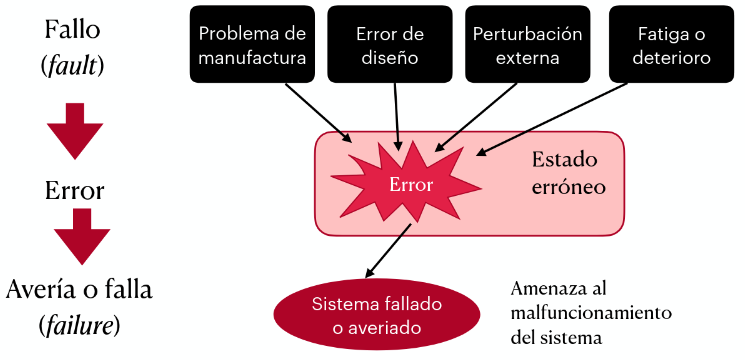
\includegraphics[width=0.48\linewidth]{img/Modelo_Causal_de_averias.png}
    \caption{Modelo Causal de averias}\label{fig:1761579857293}
\end{figure}

Pero, que causa un mal funcionamiento de un sistema. Partiremos definiendo 3 diferencias claves para el analisis.

\begin{itemize}
    \item \textcolor{red}{\textbf{Fallo(\textit{fault}):}} Defecto o funcionamiento anormal de un componente, el cual tiene el potencial de causar un \textcolor{red}{\textbf{error}}, en caso de no ser tratado \textcolor{red}{\textbf{puede llevar a una averia}}. Se clasifican segun persistencia (\textcolor{red}{\textbf{transistente, intermitente o permanente}}) y según causa \textcolor{red}{\textbf{error de manofactura, diseño u operacional}} 
    \item \textcolor{red}{\textbf{Error:}} Discrepancia entre el comportamiento esperado y el exhibido
    \item \textcolor{red}{\textbf{Averia(\textit{failture}):}} Ocurre un malfuncionamiento que conduce a que ya no se pueda proveer el servicio especificado. Son causadas por errores que se propagar a lo largo del sistema, llegando a ser observables por el usuario.
    \subitem \textbf{Un error o fallo no necesariamente conduce a una averia, si este es tratado y manejado adecuadamente}
\end{itemize}

Las \textbf{\textit{fallas}} o \textbf{\textit{averias}} se clasifican según su comportamiento en el sistema

\begin{itemize}
    \item Fallas de \textcolor{red}{\textbf{caida (\textit{crash}):}} Componente se detiene y no se recupera por si mismo
    \subitem \textcolor{red}{\textbf{Proceso:}} Proceso fallado se detiene, puede perder su estado. Es la mas benigna es detenerse manteniendo su estado, para posteriormente recuperarlo. Para la detenccion fiable por parte de otros procesos se requieren \textcolor{red}{\textit{timers}}
    \subitem \textcolor{red}{\textbf{Comunicación:}} Falla del sistema de comunicación con pérdida continua de mensajes (e.g falla permanenete o partición de red)

    \item Fallas de \textcolor{red}{\textbf{omisión:}} El sistema no responde transitoriamente
    \subitem \textcolor{red}{\textbf{Proceso:}} Proceso no responde, sin perder estado \textcolor{red}{(e.g., se pierde una solicitud de servicio)}.
    \subitem \textcolor{red}{\textbf{Comunicación:}} Se pierden algunos mensajes. Falla mas benigna es que mensajes no se corrompen (integridad) y no se puede falsear su
    remitente (autenticidad). Recuperación es por retransmisión de mensajes perdidos.

    \item Fallas \textcolor{red}{\textbf{temporales (\textit{timing}):}} El sistema no responde dentro de los limites de tiempo.
    \subitem Pueden corresponder a un mal desempeño por sobrecarga. 
    \subitem Pueden ocurrir por fallas de relojes.

    \item Fallas \textcolor{red}{\textbf{arbitrarias (\textit{bizantinas}):}} El sistema se comporta inconsistente o maliciosamente.
    \subitem Los procesos fallas siguen funcionando pero no garantizan la integridad de los mensajes \textcolor{red}{\textbf{(peor caso)}}
    \subitem A veces se produce por corrupción interna del sistema, causan respuestas erroneas pero no maliciosas
    \subitem Son fallas dificiles de detectar y tolerar
\end{itemize}

Una vez definidas el tipo de fallas, estableceremos los modelos para los tipos de fallas, en base a una jerarquia.
\begin{figure}[H]
    \centering
    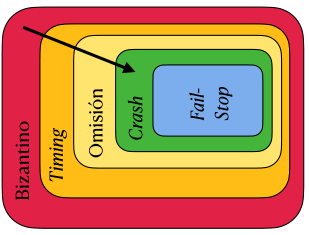
\includegraphics[width=0.3\linewidth]{img/modelo_de_fallas.png}
    \caption{Modelo jerarquico de fallas}\label{fig:1761584179354}
\end{figure}

\begin{itemize}
    \item \textcolor{red}{\textbf{Fail-stop:}} Un proceso fallado se detiene, conservando su estado, y todos los demas saben inmediatamente que ha fallado. Los procesos se comportan correctamente o se detienen.
    \item \textcolor{red}{\textbf{Crash:}} Modelo realista de incertidumbre para sistemas asincronicos. Un proceso fallad se detiene, conserva su estado, pero los demans no lo saben ni estan seguros si se cayo o esta lento o tiene problemas de comunicación. Puede recuperarse y reintegrarse al sistema
    \item \textcolor{red}{\textbf{Omisión:}} Solo un proceso puede omitir enviar o recibir mensajes. Se puede abordar con el uso de timers, reintento y asentimientos.
    \item \textcolor{red}{\textbf{Temporal (\textit{timing}):}} El sistema puede violar restricciones temporales, tal como respuestas fuera de tiempo. Dificil de discriminar entre fallas de crash y omisión
    \item \textcolor{red}{\textbf{Bizantino:}} Un proceso puede enviar mensajes contradictorios, mentir sobre su estado interno o colaborar maliciosamente con otros. Corresponde a un modelo más general
\end{itemize}

Para manejar lo anterior, se propone los siguientes enfoques para mejorar la confiabilidad del sistema.

\begin{itemize}
    \item \textcolor{red}{\textbf{Prevención de fallos:}} Prevenir que ocurran o se introduzcan fallos en el sistema
    \item \textcolor{red}{\textbf{Remoción de fallos}} durante el desarrollo o durante el uso \textbf{(mantencion y reparacion)}
    \item \textcolor{red}{\textbf{Pronóstico de fallos:}} Predecir fallos probables, para que puedan ser anticipadamente eliminadas o contener sus efectos \textbf{(e.g. alertas y detección de degradación/anomalías)}
    \item \textcolor{red}{\textbf{Pronóstico de fallos:}} Capacidad de un sistema para seguir funcionando normalmente, aun cuando seproduzcan uno o más fallos de sus componentes.
    \subitem Se debe disponer de algún tipo de redundancia para enmascarar fallos.
    \subitem Capacidad de reparar un fallo sin interrumpir el servicio, para asegurar continuidad operacional del servicio.
\end{itemize}

\subssection{Tolerancia a fallos}
Definimos la tolerancia a fallos como la capacidad de enmascarar la existencia de fallos en un sistema, usando redundacia. Esto busca evitar una averia o falla del sistema. Si bien un sistema puede ser tolerante a fallos, estos deberian ser de sus propios componentes, y no con fallas que comprometen todo el sistema. Queremos que el sistema, a pesar de que sus componentes esten fallados, este tenga un comportamiento consistente a lo especificado.
\vspace{1mm}

El manejo de fallos en un sistema es un proceso de cuatro fases: primero, la \textbf{Detección de error}, donde los fallos se deducen por errores en el estado del sistema; segundo, la \textbf{Aislación y evaluación del daño}, que busca contener la expansión del error; tercero, la \textbf{Recuperación del error}, que corrige el problema y devuelve el sistema a un estado consistente (e.g., \textit{rollback}); y finalmente, el \textbf{Tratamiento del fallo y servicio contínuo}, que, ante fallos permanentes, reconfigura el sistema para dejar de usar el componente dañado y reemplazarlo.

La \textcolor{red}{\textbf{redundancia}} se define en base a las partes de un sistema que no son necesarias para su correcto funcionamiento, si no se requiere tolerar fallos. Existen 3 tipos de tolerancias
\begin{enumerate}
    \item \textbf{Espacial:} Se agregan componentes de redundantes de hardware o software.
    \item \textbf{Temporal:} Ejecutar y repetir varias veces una acción o secuencia de instrucciones (similar a la maquina de estado determoinista y replicada). Un ejemplo es la retransmisión de mensajes, rollback de una acción y repetir su ejecición.
    \item \textbf{De información:} Se agrega información redundante para tolerar fallos.
\end{enumerate} 

\subsection{Enfoques de recuperación de errores}
Para recuperarnos de errores durante la ejecución tenemos dos enfoques.

\textbf{Recuperación regresiva(\textit{backward recovery}):} El sistema retrocede a un estado correcto anterior y se repite la ejecución, se introduce el concepto de checkpoints en la ejecución, los cuales son puntos donde se guarda el estado del sistema en una memoria estable (no se ve afectada por alguna averia). En caso de detectar errores, el sistema hace un rollback.

\textbf{Recuperación progresiva(\textit{forward recovery}):} El sistema sigue avanzando, corrigiendo un posible estado erroneo. Al detectarse errores, se siguie si ejecución mientras que a la par se realizan acciones correctivas. No es viable para todos los sistemas

\begin{figure}[H]
    \centering
    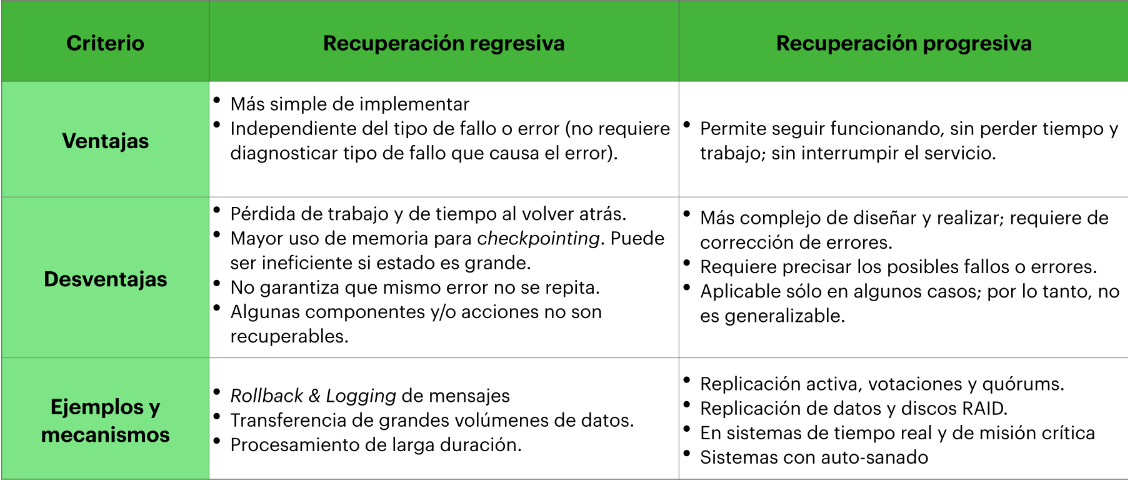
\includegraphics[width=1\linewidth]{img/Comparacion_enfoques.png}
    \caption{Comparativa de enfoques de recuperación}\label{fig:1761609494042}
\end{figure}

Dentro de los esquemas para tolerancia a fallos encontramos 
\begin{itemize}
    \item Transacciones o acciones atomicas
    \item Checkpoint y rollback
    \item Replicación de procesos
    \item Maquina de estado replicada o determoinista
    \subitem Basada en multicast atomico con orden total
    \subitem Ordenamiento basado en conceso (Paxos,Raft)
\end{itemize}

\subsection{Maquina de estado determinista y replicada}
Esta maquina es un grupo de replicación, donde cada proceso no fallado, ejecuta los mismos comandos en el mismo orden. Se caracteriza por el determinismo de estado, donde todas las replicas correctas mantienen el mismo estado. Se necesita concenso (dińamico) de los miembros del grupo, este consenso es sobre \textcolor{red}{\textbf{cúales comandos ejecutar y en que orden}}. Se trabaja sobre modelos con o sin fallas donde, si se trabaja en un modelo \textbf{sin fallas}, se pueden usar relojes de lampor para ordenamiento global y total de los mensajes del grupo o un secuenciador central. Para el caso del modelo con fallas, se requieren de algoritmos de consesso tolerantes a fallos. 

Para un ejemplo vamos a considerar lo siguiente, un contador $k$, el cual es iniciado con un valor de 1, tendremos dos maquinas que ejecutaran las mismas instrucciones, pero en diferente orden, para este caso:

\textcolor{red}{\textbf{Maquina A:}}
\begin{itemize}
    \item Multiplicar por 2 a $k$
    \item Sumarle 1 a $k$
\end{itemize}
\textcolor{red}{\textbf{Maquina B:}}
\begin{itemize}
    \item Sumarle 1 a $k$
    \item Multiplicar por 2 a $k$
\end{itemize}
\vspace{1mm}

Esto resulta en que al final el contador de la maquina A, sera \textcolor{red}{$k=3$} y para la maquina B, el \textcolor{red}{$k=4$}. por esto buscamos mantener un orden y los mismos comandos para ambas maquinas.

\subsection{Modelos cuantitativos de confiabilidad}


%Pagina 21







%Pagina 44

%seguir aqui!!!!